\chapter{Elements of Audio Signal Processing}\label{ch:processing}
\openepigraph{Signal, a function that conveys information about a phenomenon.
$[\dots]$ Consider an acoustic wave, which can convey acoustic or music information.}{R. Priemer, \textit{Introductory Signal Processing}}
\vspace{-2.5em}
\newthought{Synopsis} Let us now move from the physic to digital signal processing.
At first this chapter formalized fundamental concepts of audio signal processing such as signal, mixtures and noise~\cref{sec:processing:model}.
Secondly, this concepts representation~\cref{sec:processing:domains}
The notation presented in this chapter is reported in~\cpageref{ch:notation}, and is inspired to the one used in \citeonly{gannot2017consolidated}.


\section{Signal model in the time domain}\label{sec:processing:model}
In the previous chapter we formalized the physics that rule the sound propagation from the source 'till the microphone.
The protagonist of this chapter is the audio signal.
A raw \textit{audio signal} encodes the variation of pressure over time on the microphone membrane.
Mathematically it is denoted as the function
\begin{center}
    $x(t)$
    ,
\end{center}
continuous both in time $t \in \R$ and in amplitude $x(t_0) \in \R$.

Today signals are processed, stored and analyzed by computer and modules in their digital representation.
In short, the \textit{digital audio signal} is obtained from an analog signal in two steps:
first, the continuous time signal $x(t)$ is converted to a discrete time series,
so that $x[n]$ with $n \in \Z$ is \textit{sampled}\sidenote{
   Please note, that the use of the word \textit{sample} will have different
   meanings in the context of machine learning, where a sample is an instance of a full signal instead of a single time
}  with equidistant steps $\Ts\;[\si{\second}]$, called sampling period;
secondly, the amplitude values can be \textit{quantized}.
At the end of the digitalization process, $x[n] \in \R$ with $n = 0, \dots, N-1$, represents a one dimensional time series of amplitudes.
It is important to notice that this series is finite, with $N$ values.
This process can be modeled in two stage: first, the continuous-time signal undergoes a (ideal) low-pass filter
limiting the signal frequencies to at max $\Fs$; secondly, it is regularly sampled at rate $\Fs$.
By using the (ideal) low-pass filter $\lowpassfilter$\sidenote{
    The low-pass filter is used to reduce aliasing (spectral components higher than Fs)
    $\lowpassfilter(t) = \sinc(t) = \sin(\pi t) / (\pi t)$.
} with frequency support $\kintervoc{\sfrac{-\Fs}{2}}{\sfrac{\Fs}{2}}$,
this processes writes:
\begin{equation}
    x[n] = (\lowpassfilter \conv x)\kparen{\frac{n}{\Fs}}
    \mathspace
    \kforall[n = 0, \cdots, N-1]
\end{equation}
where $\Fs = \sfrac{1}{\Ts}\;[\si{\Hz}]$ is the \textit{sampling frequency}.
\\The choice of $\Fs$ depends massively on the application since it translates into a trade-off between computational power, sound and processing quality.
Historically two iconic values are $\SI{44.1}{\kHz}$ for music distribution on CDs and $\SI{8}{\kHz}$ for first-generation speech communication.
Now multiple of $\SI{8}{\kHz}$ are typical chosen values: ($16, 48, 96, \SI{128}{\kHz}$).
\\For further details, we refer the reader to audio signal processing basics books such as~\cite{rocchesso2003introduction}.

\newthought{Audio Signals are emitted by Sources} and are observed, received or recorded by microphones.
A set of microphones is called a microphone \textit{array}, whose element is sometime referred to as \textit{channel}.
In this thesis, these objects are assumed to have been deployed in a indoor environment, a room.
\begin{center}
    \textit{All of these make our indoor \emph{auditory scene}.}
\end{center}
Before describing the mixing process, let us provide some taxonomy, through some dichotomies:

\dichotomy{Sources \vs/ Mixtures:}
Sound sources emits sounds.
When multiple sources are active at the same time, the sound that reaches our ears or is recorded using a microphone is superimposed or \textit{mixed} to a single sound.
The \textit{mixture} represents this (set of) signal which are also denotes as channel(s).

\dichotomy{Single-Channel \vs/ Multichannel:}
The term \textit{channel}
\sidenote{
    Please note, the term \textit{channel} has also different meaning:
    it indicates the medium in communication (\eg/ Channel Estimation)
    and sometimes one of the dimension of the input in machine learning (\eg/ image's channel)
} is used here to indicate the output of one microphones or one source.
A \textit{single-channel} signal ($\numMics = 1$) is represented by the scalar $\mic(t) \in \R$,
while a \textit{multichannel} ($\numMics >   1$) is represented by the vector.

\dichotomy{Point \vs/ Diffuse Sources:}
\textit{Point sources} are emitted by a single and well-defined point in the space and their signal is single-channel.
Point sources are for instance human speakers or the sound emitted by a loudspeaker.
\\\textit{Diffuse sources} refers for instance to wind, traffic noise, or large musical instruments, which emit sound in a large region of space.
Their sound cannot be associate to a punctual source, but rather a distributed (infinite) collection of them.

\dichotomy{Directional \vs/ Onmidirectional:}
An \textit{omnidirectional} source (\resp/ receiver) will in principle emit (\resp/ pick up) sound equally from all directions,
with respect both time and frequency.
Although this simplify greatly processing frameworks, this is not true in real scenario.
The physical properties of real sources (\resp/ receivers) leads to \textit{directivity patterns}, \aka/ \textit{polarity}, which may
be different at different frequencies.
This effect may be a source of undesired effects, such as microphones \textit{leakage} or source localization error.
Nevertheless sometimes it can be exploited to promote \textit{spatial selectivity}:
spatial filtering can be view under this light, where ``virtual'' microphones with engineered directivity pattern.

\subsection{The Mixing Process}
Let us assume the observed signal has $\numMics$ \textit{channels} indexed by $\idxMic \in \kbrace{1,\dots,\numMics}$,
$\mics(t) = \ktranspose{\klist{\mic_1(t), \dots, \mic_{\numMics}(t)}} \in \R^{\numMics \times 1}$.
Let us assume that there are $\numSrcs$ sources indexed by $\idxSrc \in \numSrcs$.
Each microphone $\idxMic$ and each source $\idxSrc$ have a well defined position in the space, $\positionMicrophone_\idxMic$, $\positionSource_\idxSrc$, respectively.

The mixing process describes then the nature of the mixtures.
In order to better formalized it, \citeauthor{sturmel2012linear} introduced an intermediate representation:
\begin{center}
    \textit{The \emph{source spatial images} $\img_{\idxMic\idxSrc}(t)$ describes the contribution of the
    \\source $\idxSrc$ to the microphone $\idxMic$, and
    \\the \emph{mixture} $\mic(t)$ is the possibly non-linear combination of images.}
\end{center}
% In math,
% \begin{equation}
%     \img_{\idxMic\idxSrc}(t) &=  \kparen{g_{\idxMic\idxSrc} \conv \src_\idxSrc} (t)
%     ,
% \end{equation}
% where $g_{\idxMic\idxSrc}$ is a generic filter proper of source $\idxSrc$ and microphone $\idxSrc$.
Depending on the ``contribution'' the image describes, the following type of mixture can be defined:

\dichotomy{Natural \vs/ Artificial Mixtures:}
The former refers to microphone mixtures recorded simultaneously the same auditory scene, \eg/ teleconferencing systems or hands-free phones.
By contrast, the latters are created by mixing together different individual, possibly processed, recordings.
This are the typical mixtures used professional music production\sidenote{here the usage of long-chain of audio effects typically ``hide'' the recoding environment of the sound sources}.

\dichotomy{Instantaneous \vs/ Convolutive Mixtures:}
In the fist case, the mixing process boils down to a simple linear combination of the source signals, namely
the mixing filters are just scalar factors.
This is the typical scenario when sources are mixed using a mixing console.
\marginpar{%
        \footnotesize
        \centering
        \begin{tabular}{p{0.33\linewidth}|p{0.66\linewidth}}
        \toprule
        instantaneous   & $x_{i} \ =\sum ^{J}_{j=1} a_{ij} s_{j} $ \\
        anechoic        & $x_{i} \ =\sum ^{J}_{j=1} a_{ij} s_{j}( t - \tau _{ij}) $ \\
        convolutive     & $x_{i} \ =\sum ^{J}_{j=1}( g_{ij} \ast s_{j})( t)$ \\
        \bottomrule
        \end{tabular}
        \captionof{table}{Taxonomy of linear mixing models for a mixture channel $x_i$, sources $s_j$, impulse response $g_{ij}$,
        scaling factor $a_{ij}$ and delay $\tau_{ij}$.}
}
Convolutive mixtures, instead, denote the more general case where the each mixture is the sum of filtered signals.
In between are the \textit{anechoic} mixtures involving the sum of scaled and delayed source signals.

With this being said, natural mixtures are convolutive by nature and ideal free-far-field natural recording are well approximated by anechoic mixtures.
In this thesis, we will particularly focus on natural mixture which exhibits a natural correspondence between image sources, impulse responses and the
room properties of the auditory scene.

% Being $\spat_\idxSrc(\cdot)$ a possibly nonlinear spatialization operation, the spatial images
% $\imgs_\idxSrc(t) = \ktranspose{\klist{\img_{1\idxSrc}(t), \dots, \img_{\numMics\idxSrc}(t)}}$ with respect to the $\numMics$ reads
% \begin{equation}
%     \imgs_\idxSrc(t) = \kbracket{\spat_\idxSrc(\idxSrc)}(t)
%     .
% \end{equation}
% In second stage, the images of all (point and diffuse) sources are added together and passed through a possibly
% nonlinear \textit{post-mixing} operation $\master(\cdot)$ to obtain the mixture signal $\mics(t)$
% \begin{equation}
%     \mics(t) = \kbracket{ \master\kparen{
%                     \sum_{\idxSrc=1}^{\numSrcs} \imgs_\idxSrc
%                     }}(t)
% \end{equation}
% \marginpar{
%     \footnotesize
%     In the field of music productions,
%     $\spat_\idxSrc(\cdot)$ and $\master(\cdot)$ may be identify rispectively with the \textit{mixing} and \textit{mastering} process.
% }

\begin{figure}[t]
    \begin{fullwidthfig}
        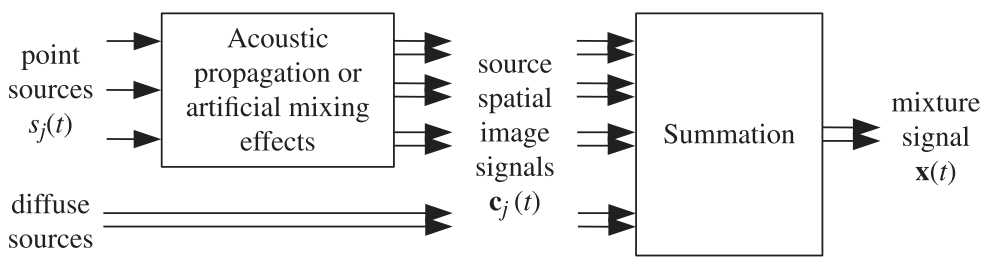
\includegraphics[width=\linewidth+\marginparsep]{processing/mixing_process.png}
    \end{fullwidthfig}

    \vspace{-\baselineskip}\vspace{-\baselineskip}
    \sideparmargin{outer}
    \sidepar{\vspace{\baselineskip}
    \caption{General mixing process, illustrated in the case of $\numSrcs = 3$ sources,
      including three point sources and one diffuse source, and $\numMics = 2$ channels.}
    }
    \label{fig:processing:mixing}
\end{figure}

\newthought{In context of room acoustics}, the microphone mixture listen to the propagation of sound in the auditory scene.
As discussed in~\cref{ch:acoustics:sec:wave}, this process is linear (and time invariant provided a static scenario).
% In this case, the spatialization operation $\spat_\idxSrc(\cdot)$ is expressed by
% collection of convolution with \RIR/ $h_{\idxMic\idxSrc}$
% from source $\idxSrc$ to microphone $\idxMic$ and the post-mixing operation $\master(\cdot)$ reduces to the identity:
Therefore, the resulting mixture is the simple summation of the sound images,
which are the collections of convolution between the \RIRs/ and source signal:
\marginpar{
    \centering
        \tikzset{every picture/.style={line width=0.75pt}} %set default line width to 0.75pt
        \resizebox{\linewidth}{!}{
            \begin{tikzpicture}[x=0.75pt,y=0.75pt,yscale=-1,xscale=1]

                % Picture Node
                \draw (333,148.65) node  {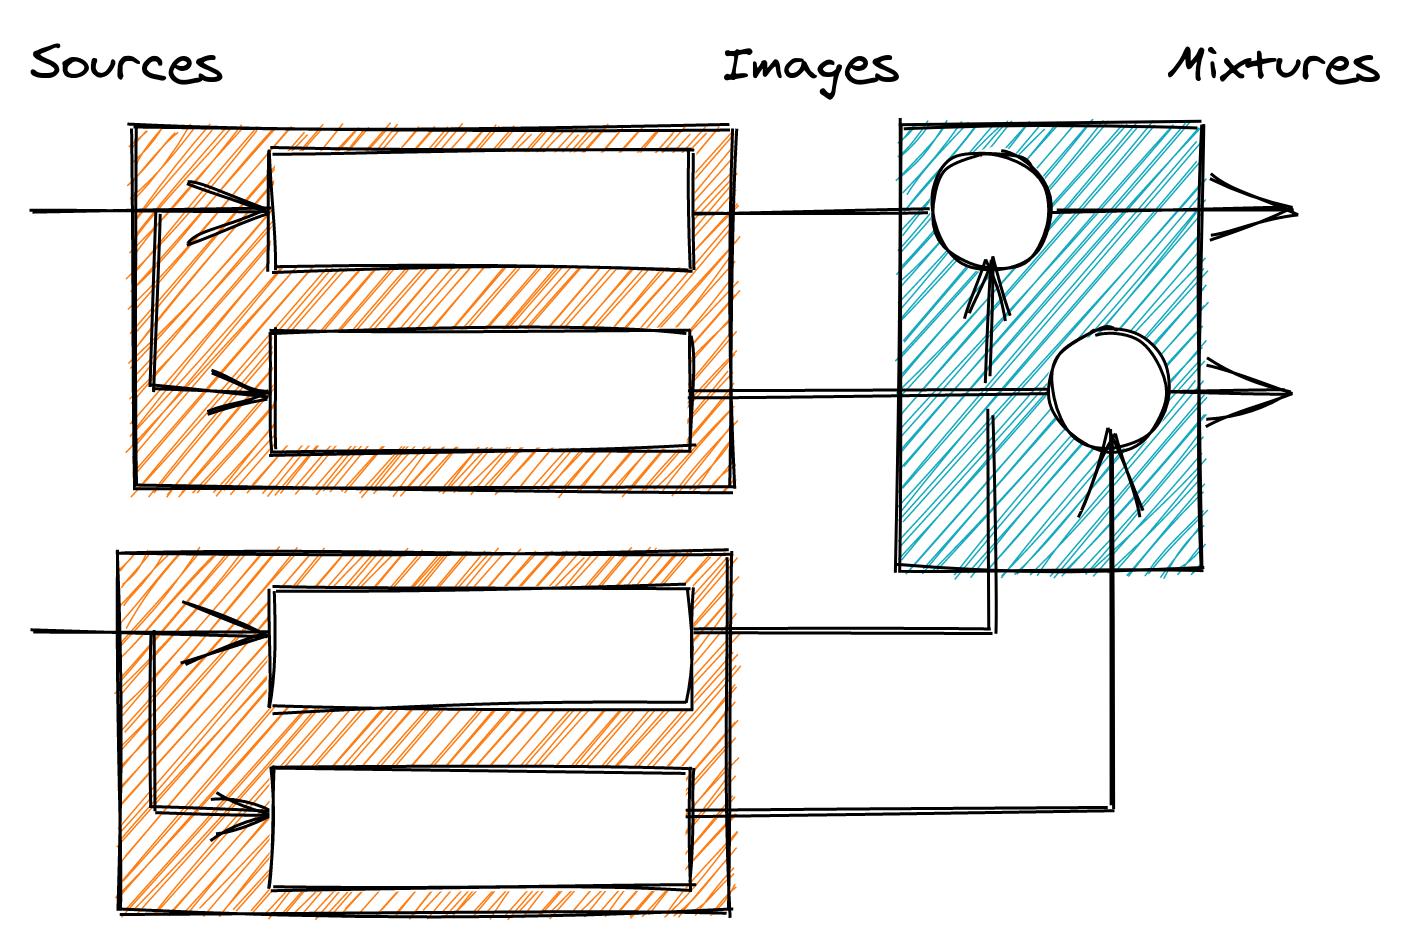
\includegraphics[width=333.75pt,height=222.97pt]{processing/mixing_blocks.png}};

                % Text Node
                \draw (126,53) node [font=\huge]   {$s_{1}$};
                % Text Node
                \draw (126,183) node  [font=\huge]  {$s_{2}$};
                % Text Node
                \draw (262,63) node  [font=\huge]  {$h_{11} \ast s_{1}$};
                % Text Node
                \draw (262,120) node  [font=\huge]  {$h_{21} \ast s_{1}$};
                % Text Node
                \draw (370,53) node  [font=\huge]  {$c_{11}$};
                % Text Node
                \draw (370,110) node [font=\huge]   {$c_{21}$};
                % Text Node
                \draw (530,53) node   [font=\huge] {$x_{1}$};
                % Text Node
                \draw (530,110) node  [font=\huge]  {$x_{2}$};
                % Text Node
                \draw (262,199) node  [font=\huge]  {$h_{12} \ast s_{2}$};
                % Text Node
                \draw (262,256) node  [font=\huge]  {$h_{22} \ast s_{2}$};
                % Text Node
                \draw (370,183) node  [font=\huge]  {$c_{12}$};
                % Text Node
                \draw (370,240) node   [font=\huge] {$c_{22}$};
                % Text Node
                \draw (412,53) node [anchor=north west][inner sep=0.75pt]  [font=\huge]  {$\sum $};
                % Text Node
                \draw (448,109) node [anchor=north west][inner sep=0.75pt]  [font=\huge]  {$\sum $};

            \end{tikzpicture}
        }
        \captionof{figure}{Graphical representation of the mixing model~\ref{eq:processing:mixing} for 2 sources and 2 microphones.}\label{fig:processing:mixing}
}
\begin{align}
    \img_{\idxMic\idxSrc}(t) &=  \kparen{h_{\idxMic\idxSrc} \conv \src_\idxSrc} (t)     \label{eq:processing:mixing:img} \\
    \imgs_\idxSrc(t) &= \ktranspose{\klist{\img_{1\idxSrc}(t), \dots, \img_{\numMics\idxSrc}(t)}} \nonumber\\
    \mics(t)         &= \sum_{\idxSrc=1}^{\numSrcs} \imgs_\idxSrc(t)                    \label{eq:processing:mixing:mix}
\end{align}%
where $\conv$ is the linear convolution operator.
Considering the time domain description of the \RIR/ derived (and approximated) in the previous chapter\sidenote{\cfr{\cref{eq:acoustics:rir_full,eq:acoustics:ims}}},
the time-domain \emph{mixing filters} $h_{ij}( t)$ will be modeled as follows:
\begin{equation}\label{eq:processing:mixing_filter}
    h_{ij}( t) = \sum_{\idxEch=0}^{\numEchs} \frac{\absCoeff_{ij}^r}{4 \pi \speedOfSound \tau_{ij}^r}
                       \diracOf{t - \tau_{ij}^r} + \varepsilon_{ij}(t)
\end{equation}
where $\absCoeff_{ij}^r$ and $\tau_{ij}^r$ are the attenuation coefficient and the time delay of the reflection $\idxEch$.
The noise term $\varepsilon_{ij}( t)$ collects later echoes ($\idxEch > \numEchs$) and the tail of the reverberation.
We do not assume $\varepsilon_{ij}( t)$ to be known.

\subsection{Noise, interferer and errors}
\openepigraph{%
    \emph{Noise} is a general term for unwanted (and, in general, unknown) modifications that a signal may suffer during capture, storage, transmission, processing, or conversion
}{V. Tuzlukov, \textit{Signal processing noise}}
In~\cref{eq:processing:mixing:mix} no noise is included:
all the sources are threated in the same way, including \textit{target}, \textit{interfering} and \textit{noise} sources.
In~\cref{eq:processing:mixing_filter} a noise term is added to collects unknown quantities.
Noise has then different meanings.
While the definition of target sound source is quite self-explanatory and it will denoted as the source $j = 1$,
the term interfer and noise depends on the specific use case, problem, application, and research field.
With this being said, we will define and use the following type of noises:
\newthought{Interfers} identifies the undesired source with properties similar to the target source.
For instance, a concurrent speech source for speech application or concurrent music instrument in case of music.
\\In this thesis, and in particular in~\cref{chap:dataset,chap:brioche}, the interfer sources will be denoted
as additional source indexed by $j > 1$.
\marginpar{
    \centering
        \resizebox{\linewidth}{!}{
            \begin{tikzpicture}[x=0.75pt,y=0.75pt,yscale=-1,xscale=1]
            \draw (346.67,226.03) node  {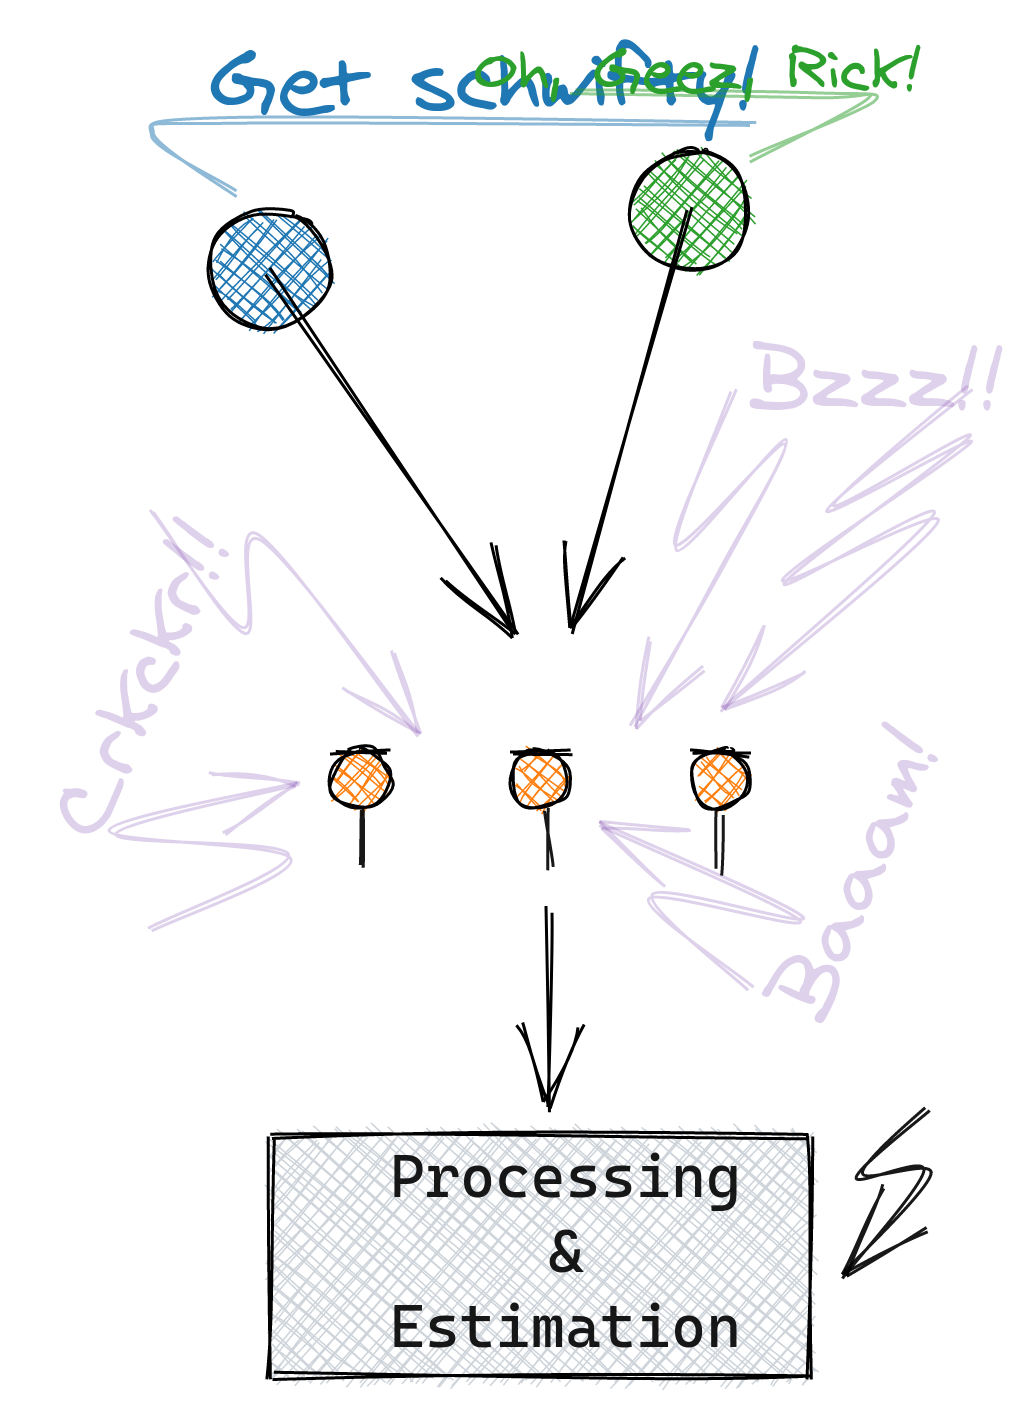
\includegraphics[width=246.25pt,height=335.73pt]{processing/noise.png}};
            % Text Node
            \draw (203.5,100.4) node [anchor=north west][inner sep=0.75pt]  [font=\Large]  {$s_{1}( t)$};
            % Text Node
            \draw (429.5,49.9) node [anchor=north west][inner sep=0.75pt]  [font=\Large]  {$s_{2}( t)$};
            % Text Node
            \draw (455.5,196.9) node [anchor=north west][inner sep=0.75pt]  [font=\Large]  {$\boldsymbol{n}( t)$};
            % Text Node
            \draw (308.5,285.9) node [anchor=north west][inner sep=0.75pt]  [font=\Large]  {$\boldsymbol{x}( t)$};
            % Text Node
            \draw (465.5,327.4) node [anchor=north west][inner sep=0.75pt]  [font=\Large]  {$\boldsymbol{\varepsilon }( t)$};
            \end{tikzpicture}
        }
        \captionof{figure}{Graphical representation of the mixing model~\ref{eq:processing:mixing}:
        $s_2(t)$ is the \textit{interferer},
        $\boldsymbol{n}( t)$ contributes to the \textit{diffuse noise field}, and
        $\boldsymbol{\varepsilon }( t)$ model acquisition and modeling errors.
        }\label{fig:processing:mixing}
}
\newthought{Noise} collects all the remaining effects, typically nonspeech sources. Moreover we will make a further distinction:

\newthought{Diffuse Noise Field} describes the background diffuse sources present in the auditory scene, such as car noise, indistinct talking or winds.
It can be modeled as \AWGNdef/, but its spatial description must be taken into account\citeonly{habets2007generating}.
\\In this thesis, it is denoted as $\bsn(t) \sim \calN(0, \cov_{nn})$ where $\cov_{nn} \in \bbR^{I \times I}$ is the noise \textit{spatial covariance matrix}

\newthought{Measurement and Model Noise} accounts for general residual miss- and under-modeling error.
As common is signal processing and information theory, this error term will be modeled as \AWGN/.
\\In this thesis, it will denoted as $\varepsilon_{ij}( t)$ will be used to model residuals and measurement error,
\eg/ approximation of the \RIR/ with the \ISM/ or sensor noise, respectively.

\medskip\noindent
Making the noise terms and sources explicit, the mixing model in~\cref{eq:processing:mixing:img,eq:processing:mixing:mix} writes:
\begin{align}
    \img_{\idxMic\idxSrc}(t) &=  \kparen{h_{\idxMic\idxSrc} \conv \src_\idxSrc} (t) +  \varepsilon_{ij}(t)\\
    \imgs_\idxSrc(t)         &= \ktranspose{\klist{\img_{1\idxSrc}(t), \dots, \img_{\numMics\idxSrc}(t)}} \nonumber\\
    \mics(t)                 &= \sum_{\idxSrc=1}^{\numSrcs} \imgs_\idxSrc(t) + \bsn( t)
\end{align}%


\section{Signal Model in the Spectral domains}\label{sec:processing:domains}
The frequency, or spectral, representation is probably the most famous signal representation used in signal processing
\sidenote{%
It was introduced by Joseph Fourier in his work on the heat equation~\citeonly{fourier1822theorie}.
His mathematical tool, named later \textit{Fourier Decomposition},
aims at approximating any signal by a sum of sine and cosine waves.}.
Here speech and music signals, which naturally exhibit harmonic and periodic behaviors,
are described as combination of sinusoids as function of their frequencies.
% https://tex.stackexchange.com/questions/127375/replicate-the-fourier-transform-time-frequency-domains-correspondence-illustrati

This operation is achieved through the \FTdef/, $\fourierTrans{}:\bbR\kmapsto\bbC$, which
project a continuous-time-domain signal $x$ onto a space spanned by continuous-frequency complex exponentials:
\begin{equation}\label{eq:processing:ft}
    x(f) = (\fourierTrans{x})(f) =
        \int_{-\infty}^{+\infty}
        x(t)
        \cste^{-\csti 2 \pi f t}
        \,\kdiff{t}
    ,
\end{equation}
where $f \in \bbR$ are the \textit{natural frequency} in $\si{\Hz}$ and $\csti$ is the imaginary unit.

A part from providing a space where audio signal reveals their harmonic structures, the Fourier transforms benefits of two fundamental properties:
it is linear and it converts time-convolution into element products.
\\First, linearity allows to write~\cref{eq:processing:mixing:mix} simply as:
\begin{equation}\label{eq:processing:ft:mix}
    \mics( t) = \sum_{\idxSrc=1}^{\numSrcs} \imgs_\idxSrc( t)
    \;\overset{\fourierTrans{}}{\rightarrow}\;
    \mics( f) = \sum_{\idxSrc=1}^{\numSrcs} \imgs_\idxSrc( f)
\end{equation}
Secondly, by the \textit{convolution theorem}, the source spatial images in~\cref{eq:processing:mixing:img} writes as:
\begin{equation}\label{eq:processing:conv}
    \img_{\idxMic\idxSrc}( t) =  \kparen{h_{\idxMic\idxSrc} \conv \src_\idxSrc} ( t)
    \;\overset{\fourierTrans{}}{\rightarrow}\;
    \img_{\idxMic\idxSrc}( f) =  h_{\idxMic\idxSrc}( f) \src_\idxSrc( f)
\end{equation}

Notice that here both $f$ and $t$ are continuous and infinite variables, so the support of the signals.
In practice, we work with finite and discrete-time signals for which the properties~\eqref{eq:processing:conv} is not valid in general.
\\As discussed in~\cref{chap:acoustics}, the \FT/ of a \RIR/, $h_{ij}( f)$
can be computed in closed-form with some approximation\sidenote{
    \cfr{\cref{eq:acoustics:ims,eq:processing:mixing_filter}}
}
\begin{equation}\label{eq:processing:rir:ft}
    h_{ij}( f) = \sum_{\idxEch=0}^{\numEchs}
                    \frac{\absCoeff_{ij}^r}{4 \pi \speedOfSound \tau_{ij}^r}
                    \cste^{- \csti 2 \pi f \tau_{ij}^r}
    .
\end{equation}
However, the \FT/ of the mixtures, $x_i( f)$, in not available due to the measurement process of sampling.

\subsection{Discrete Frequency domain}
The discrete-finite-frequency domain representation of a discrete-finite-time signal $x[n]$ is given by its (forward) \DFTdef/, $\discreteFT{}:\bbR\kmapsto\bbC$
\sidenote{
    Please note that the notation for applying the \DFT/ is the one used for matrices.
    In fact, the \DFT/ can be efficiently implemented as a matrix multiplication operation.
    Its most famous implemention is called \FFT/.
    \\This can be intrepreded as the projection onto the space spanned by a finite number of complex exponentials.
}:
\begin{equation}\label{eq:processing:dft}
    x[k] = (\discreteFT{x})[k] =
    \sum_{n = 0}^{N - 1}
    x[n]
    \cste^{-\csti2\pi k n / F}.
\end{equation}
where $k \in \kintervcc{0}{F - 1}$ in the discrete \textit{frequency bin} and $F$ is the total number of bins.
The natural frequency $f_k$ in $\si{\Hz}$ correspondent to the $k$-th frequency bin as:
\begin{equation}
    f_k = \frac{k}{F}\Fs
    .
\end{equation}

In practice, the \DFT/ is used as valid approximation of the \FT/ for the measurement
\begin{equation}
    \fourierTrans{(\lowpassfilter \conv x_i)} (f_k) \approx x_i[k]
    ,
\end{equation}
and this approximation become arbitrarily precise as the number of samples $N$ grows to infinity.

By the linearity of the \DFT/, \cref{eq:processing:ft:mix} simply translates
\begin{equation}\label{eq:processing:ft:mix}
    \mics( f) = \sum_{\idxSrc=1}^{\numSrcs} \imgs_\idxSrc( f)
    \;\leadsto\;
    \mics( k) = \sum_{\idxSrc=1}^{\numSrcs} \imgs_\idxSrc( k)
\end{equation}


As explained~\cite{tukuljac2018mulan}, particular emphasis should be paid when approximating~\cref{eq:processing:mixing:img},
since we will make use to the closed-form \FT/ of the \RIR/, $h_{ij}(f)$ of~\cref{eq:processing:rir:ft}.
\begin{enumerate}
    \item\label{en:processing:dft:one}
        the discrete-correspondent of the convolution theorem is valid for \textit{circular convolution}.
    This is only approximated by the \textit{linear convolution}, which can be reasonably good when many samples are available\sidenote{reduce bundary artifacts}.
    \item\label{en:processing:dtf:two}
        Secondly, the closed-form~\cref{eq:processing:rir:ft} is true asymptotically for $N\to\infty$.
\end{enumerate}
With that being said, the following approximated model
\begin{equation}
    \underbrace{c_{ij}[n] \approx (h_{ij} \convDis x)[n]}_{\text{approx.~\ref{en:processing:dft:one}}}
    \;\overset{\discreteFT{}}{\leadsto}\;
    c_{ij}[k] \approx h_{ij}[k] x[k]
\end{equation}
where $\convDis$ is the finite-time convolution operator\sidenote{
    The finite-time convolution for two vectors $\ttu\in\bbR^L$ and $\ttv\in\bbR^D$ is
    \\$(\ttu \convDis \ttv)[n] = \sum_{l=0}^{L-1} \ttu[l] \ttv[L-1+n-j]$ for $n = 0, \cdots, D-L$
    .
}.
Notice that few approximation are made here
\begin{itemize}
    \item First, the validity of the approximation of the right-hand equation depends on the way $h_{ij}(t)$ and $s(t)$ are sampled.
    \item Secondly, \DFT/ 's correspondent of the convolution theorem applies to \textit{circular convolution}.
          However, the actual model provides for linear convolution between finite and non-periodic signals, resulting in an approximation error.
\end{itemize}

% Note that the smoothing sinc kernel φ(t) does not impact this formula, since only frequencies below fs/2 are considered.
% Importantly, both approximations in (5.11) become arbitrarily precise as the number of samples N grows to infinit

% The validity of approximation (5.5) depends on the way hm(t) and s(t) are sampled
% First, the time-domain convolution between ˆhm and ˆs has been transformed into a multiplication through the DFT.
% This would be exact for a circular convolution, but the actual model is a linear convolution between infinite and non periodic signals, resulting in an approximation error.
% Second, the formula used for ˆhm in the right hand side of (5.11) is the one that would result from the discrete-time Fourier transform (DTFT) ofhm which would require infinitely many samples N to be calculated exactly, as opposed to the DFT
%
%


While the raw audio signal encodes the amplitude of a sound as a function of time,
its Fourier spectrum represents it as a function of frequency, but los completely variation over time.
In order to jointly account for temporal and spectral characteristic, following representation is used.

\subsection{Time-Frequency domain}
\newthought{\TFdef/ Representation} aims to jointly describe the signal in time and frequency domain.
the \STFTdef/ encodes the time-varying spectra into a matrix $x(k,l) \in \bbC^{F,T}$ with frequencies $k$ and time frames $l$.

the \STFT/ has the following useful properties for audio processing~\cite{vincent2018audio}:
\begin{itemize}
    \item the frequencies scale $f$ is a linear function of the frequency bin $k$;
    \item the resulting matrix allows easy treatment of
          the phase $\phaseOf{x(k,l)}$, the magnitude $\magnitudeOf{x(k,l)}$ and the power $\powerOf{x(k,l)}$ separately;
    \item the \DFT/ can be efficienciently computed with the \FFT/ algorithm;
    \item the \STFT/ is simple to invert.
\end{itemize}

\newthoughtpar{Time-Frequency Analysis, Processing and Synthesis}
Throughout this dissertation both estimation and processing will be conducted in the  \TF/ domain.
This is a common approach in the audio signal processing community, but it is not the only one:
Many algorithm are designed directly in the time domain.
\\Along with common motivation supported by time-domain resolution or computational load requirements,
powerful machine-learning approaches are able to learn both representation and estimation steps~\cref{subsec:application:algos}.
\\In the context of \STFT/, the process of converting the signal into the \TF/-domain is called \textit{analysis}, while
its counterpart converting back to time-domain is called \textit{synthesis}.
Between the two we will conduct \textit{estimation}, \textit{processing} and \textit{enhancement}.


\section{RIR and Echoes Models}
Thanks to the convolution theorem, time-domain convolution can be implemented as a multiplication in the frequency-domain.
However this does not generalized straightforwardly to the time-frequency domain:
it depends on the length of the filter \wrt/ to the length of the analysis window on of the \STFT/.
Issues arise with long filter, which are common for microphone recoding in highly reverberant or time-varying scenarios.
To circumvent this issues, the \textit{convolutional STFT} with arbitrary analysis window have been proposed:
it implements the time-domain convolution into inter-time-frame and inter-frequency-bands products~\cref{aoe}.

In this thesis, we will assume that the filter length is much shorter than the analysis window length.
This known in the literature as the \textit{narrowband approximation}\cite{}.
\\In the time-frequency domain, $\mics_j(l,k)$  and $\src_j(l,k)$ are the \STFT/ of $\mics_j(l,k)$ and $\src_j(l,k)$ respectively.
Therefore, the time-domain filtering can be approximated by complex-valued multiplication in the STFT domain:
\begin{equation}
    \mics_j(l,k) = \bsh_j(k) \src_j(l,k)
    ,
\end{equation}
where the $\bsh_j(f) = \klist{h_{1j}(f), \cdots, h_{1j}(f)}$ is the $I \times 1$ vector of the DFT of the
\RIRs/ for the source $j$,

Recalling the derivation in~\cref{ch:acoustics:subsec:rir}, we adopt the following model for the room transfer function as:
\sidenote{\cfr{\cref{eq:acoustics:ims}}}
\begin{equation}
    \rir (k, \positionMicrophone \mid \positionSource) =
    ,
\end{equation}

\newthought{Steering Vector}
In case of absence of echoes and reverberation, namely assuming free-field propagation,
the \RIRs/ simplify to \textit{steering vector}, than is the DFT of~\cref{eq:acoustics:greenFreeTime}:
\begin{equation}\label{eq:processing:steering}
    \bsd_{j}(k) = \klist{\frac{1}{4 \pi \distMicSrc_{1j}} \cste^{-\csti 2 \pi f_k \distMicSrc_{ij} / c},
                            \cdots,
                            \frac{1}{4 \pi \distMicSrc_{Ij}} \cste^{-\csti 2 \pi f_k \distMicSrc_{Ij} / c},
                    }
\end{equation}
In far-field regimes, the microphone-to-source distance $\distMicSrc_{ij}$ are larger than the
inter-microphones distance $d_{ii'}$. Here the attenuation factors $\sfrac{1}{4 \pi \distMicSrc_{ij}}$ becomes approximately equal
and ofter are ignored.


\newthoughtpar{Relative Transfer Functions} modeled
Let us assume that the reference microphone is the first
The \RTFdef/:
\begin{equation}\label{eq:processing:rtf}
    \rtfs_j(k) = \frac{1}{\rir_{1j}(k)} \rirs_j(k)
\end{equation}

\newthought{Relative Steering Vectors} are under the free-far-field assumption on the sound propagation.
Interestingly from their closed form definition, an important geometrical property arise.
By combining~\cref{eq:processing:steering,eq:processing:rtf}, the \textit{relative steering vector} writes
\begin{equation}
    \bsd_{j}(k) = \klist{1,
                         \cste^{-\csti 2 \pi f_k \deltaTaus_{2j}},
                         \cdots,
                         \cste^{-\csti 2 \pi f_k \deltaTaus_{Ij}},
                    }
\end{equation}
where $\deltaTaus_{ij} = \frac{\distMicSrc_{ij}-\distMicSrc_{1j}}{c}$ is the \TDOAdef/.

\newthought{Interchannel Cues}
The \RTFs/ encodes the \ILDdef/ and the \IPDdef/
\begin{align}
    \ild_{ij}(k) &= 20 \log_{10} \magnitudeOf{\rtf(k)} \mathspace & [\si{\dB}]\\
    \ipd_{ij}(k) &= \phaseOf{\rtf(k)} \mathspace                  & [\si{\radian}]
\end{align}

As shown in ... the so-called \ILD/ and the \IPD/ cluster around the direct path. However early echoes and
reverberation make them significantly diverge.
\sidenote{%
    this terminology is used in the psycoacoustics fields
}


\section{Evaluation}\label{sec:evaluation}

\subsection{Signal-based metrics}
\subsection{Perceptual metrics}


\section{Data and Dataset}

\subsection{Picnic of the Muses dB}

\subsection{\dechorate}